\documentclass[main]{subfiles}

\begin{document}
	\newpage
	\subsection{Лемма о компактах в $\R^n$}

	\begin{lemma}
		$K \subset \R^n$ --- компакт, тогда:
		\begin{enumerate}
			\item K --- замкн.
			\item K --- огр.
			\item $\forall D \subset K \q D \text{ --- замкн.} \RA D \text{ --- комп.} $
		\end{enumerate}
	\end{lemma}

	\begin{Proof} \
		\center{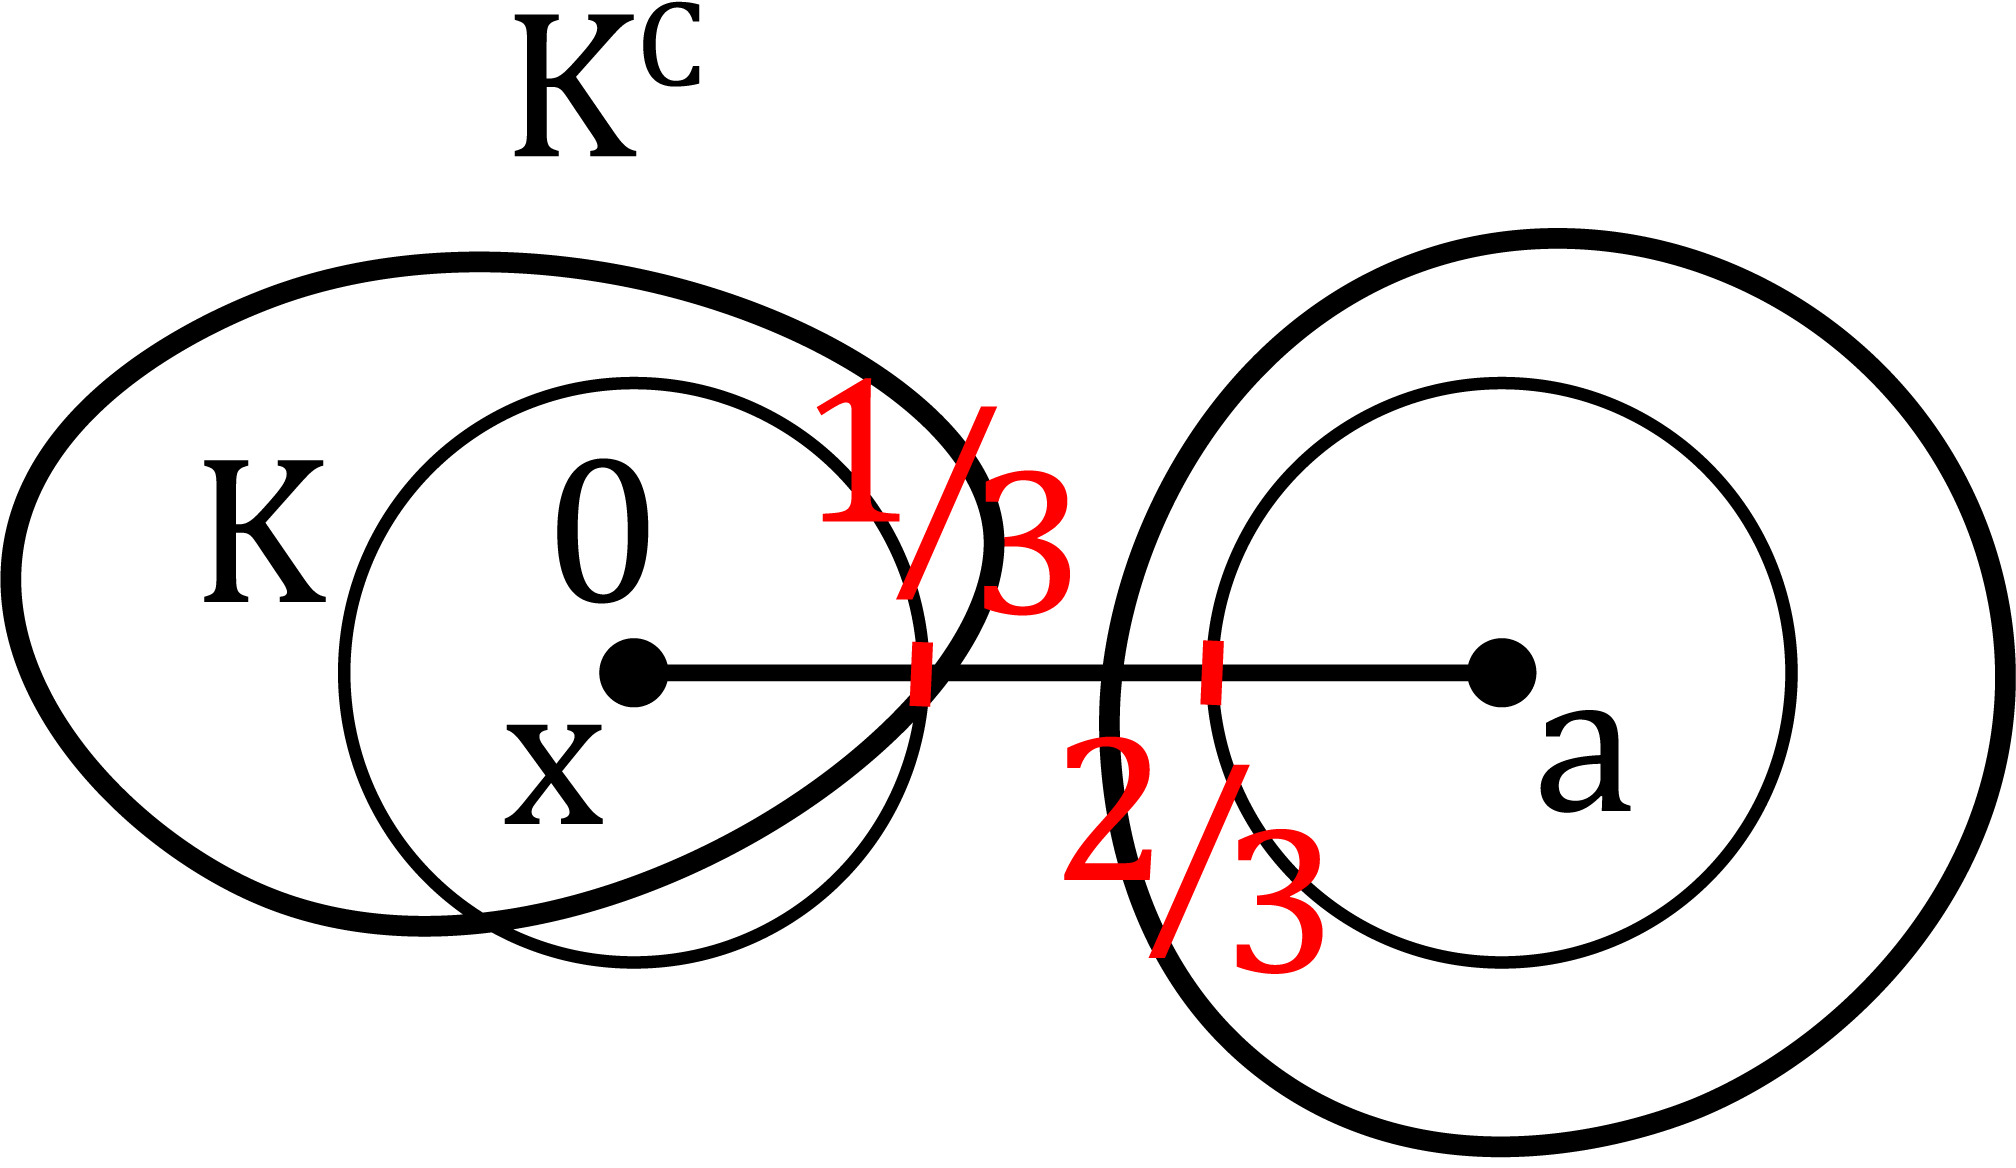
\includegraphics[width=5cm]{pics/2_1}}
		\begin{enumerate}
			\item $K^c \ni a$
			      \[\forall x \in K \q d(a, x) > 0\]
			      \[r_x = \frac{1}{3} d(x, a)\]
			      \[\forall x \in K \q B(x, r_x) \text{ --- откр.}\]
			      \[K \subset \bigcup_{x \in K} B(x, r_x) \text{ --- откр. покр. компакта } K\]
			      \[\Ra \e x_1, ..., x_N \in K : K \subset \bigcup_{j = 1}^N B(x_j, r_{x_j})\]
			      \[a \in \bigcap_{k = 1}^N B(a, r_{x_k}) = B(a, r_{\min})\]
			      \[r_{\min} = \min(r_{x_1},\ ...,\ r_{x_N}) > 0\]
			      \[\text{Причем } \bigcap_{1}^N B(a, r_{x_k}) \text{ не имеет общих точек с } \bigcup_{1}^N B(x_k, r_{x_k})\supset K\]
			      \[\e B(a, r_{\min}) \subset K^c \RA K^c \text{ --- откр. }\RA \text{K --- замкн.} \]
			\item $\us{\text{комп.}}{K} \subset \us{\text{откр. покр.}}{\bigcup_{k = 1}^\infty B(0, k)}$
			      \[\Ra \e k_1, ..., k_n\]
			      \[K \subset \bigcup_{j = 1}^N B(0, k_j) = B(0, \max_{1 \leq j \leq N}(k_j)) \RA K \text{ - огр} \]
			\item $\us{\text{замкн.}}{D} \subset \us{\text{комп.}}{K}$
			      \[\text{Пусть откр. покр. } D \subset \bigcup_{\alpha \in A} U_\alpha \]
			      \[U^* = D^c \text{ --- откр. --- добавим к покр. D}\q \{U_\alpha\}_{\alpha \in A}\]
			      \[\Ra \text{ выд. конечн. подпокр. } K \q \{U_{\alpha_j}\}_{j = 1}^N \cup \{U^*\} \]
			      \[\Ra D \subset \bigcup_{j = 1}^N U_\alpha\]
		\end{enumerate}
	\end{Proof}

	\newpage
	\subsection{Критерий компактности в $\R^n$}

	\begin{theorem}
		Следующие условия равносильны:
		\begin{enumerate}
			\item K --- компакт.
			\item K --- замк. и огр.
			\item $\forall \{x_m\}_{m = 1}^\infty \ x_m \in K$
			      \[\e \text{ подпосл } x_{m_k} \to x \in K\]
		\end{enumerate}
	\end{theorem}

	\begin{proof}
		$(1 \Ra 2)$:
		\[\text{Было}\]
		$(2 \Ra 1)$:
		\[\text{т.к. } K \text{ --- огр.} \RA \e I = \prod_{j = 1}^n [a_j, b_j], \text{ такое что}\]
		\[\text{замкн. --- }K \subset I \text{ --- комп.}\]
		\[\Ra \text{ (лемма) K --- комп.}\]
		$(2 \Ra 3)$:
		\[x_m \in K \text{ --- замкн. и огр.}\]
		\[\Ra \e x_{m_k} \text{ --- сх. (пр. выб. Б-В)}\]
		\[x_{m_k} \to x \text{ предпол. } x \not \in K\]
		\[x \in K^c \text{ --- откр. } \Ra \e B_x \subset K^c\]
		\[\text{Но }d(\us{\in K}{x_{m_k}}, x) \to 0 \text{ противоречит } x \in K \]
		$(3 \Ra 2)$:
		\[\text{а) предп. } K \text{ не явл. огр.} \]
		\[\forall n \in \N \q \e x_n \in K: d(0, x_n) > n\]
		\[\{x_n\} \text{ не огр.} \Ra \text{ не сх.}\]
		\[\Ra K \text{ --- огр.}\]
		\[\text{б) предп., что } K \text{ --- не явл. замкн.}\]
		\[K^c \text{ - не откр. }\]
		\[\e a \in K^c : \forall \delta > 0 \  B(a, \delta) \cap K \neq \varnothing\]
		\[\e x_n \in B(a, \frac{1}{n}) \cap K\]
		\[x_n \in K\]
		\[0 \leq d(x_n, a) < \frac{1}{n} \to 0 \RA x_n \to a\]
		\[\text{Из 3: }x_{n_k} \to x \in K, \text{ т.е. $a \in K$, но $a \in K^C$}\]
	\end{proof}

	\begin{Upr}
		\[K_1 \supset K_2 \supset ...\]
		\[\text{д-ть } \bigcap_{j \in \N} K_j \neq \varnothing\]
	\end{Upr}

	\newpage
	\subsection{Непрерывные отображения, эвивалентность двух определений}

	\begin{Definition}
		\[E \subset \R^n,\q f: E \to \R^m \text{ --- отобр-е (вект. ф-я)}\]
		\[(m = 1 \text{ --- ф-я})\]
		\[f(x) = (f_1(x), ..., f_m(x))\]
		\[x= (x_1, ..., x_n) \q f_j: E \to \R \text{ --- коорд. ф-я}\]
	\end{Definition}

	\begin{Definition}
		\[a \in \R^n \text{ --- пред. т. E, если:}\]
        \[\forall \delta > 0 \q \doted{U}(a, \delta) \cap E \neq \varnothing\]
	\end{Definition}

	\begin{Definition}
		\[f: E \to \R^m, a \text{ --- пред. т. E}\]
		\[\lim_{x \to a} f(x) = L \text{, если:}\]
		\[\text{(Коши) } \forall \E > 0 \q \e \delta > 0 : \forall x \in E\]
		\[0 < d(x, a) < \delta \RA d(f(x), L) < \E\]
		\[\text{(Гейне) } \forall \{x_k\}_{k = 1}^\infty \q x_k \in E \setminus \{a\} x_k \us{k \to \infty}{\to} a  \RA f(x_k) \us{k \to \infty}{\to} L \]
	\end{Definition}

	\begin{upr}
		Эквивалентность определений по Коши и по Гейне
	\end{upr}

	\begin{upr}
		Сходимость $\lra$ покоординатная сходимость
	\end{upr}

	\begin{Example}
		\[f(x, y) = \left\{ \begin{align}
				 & \frac{xy}{x^2 + y^2}, & (x,y) \neq (0, 0) \\
				 & 0,                    & (x,y) = (0, 0)
			\end{align}\]
		Повторные пределы
		\[\lim_{x \to 0} \lim_{y \to 0} f(x, y) = 0\]
		\[\lim_{y \to 0} \lim_{x \to 0} f(x, y) = 0 \]
		\[f(\delta, \delta) = \frac{1}{2} \underset{\delta \to 0}{\to}\frac{1}{2}\]
		\[f(\delta, -\delta) = -\frac{1}{2}\]
		\[\text{т.е } \lim_{(x, y) \to (0,0)} f(x, y) \text{ не сущ.} \]
	\end{Example}

	\begin{Theorem}[предел композиции]
		\[E \subset \R^n, \q F \subset \R^m, \q \R^n \ni a \text{ --- пред. т. E}, \q F \ni b \text{ --- пред. т. F}\]
		\[f: E \to F, \q g: F \to \R^l\]
		\[\lim_{x \to a} f(x) = b, \q \lim_{x \to b} g(x) = g(b) \]
		\center{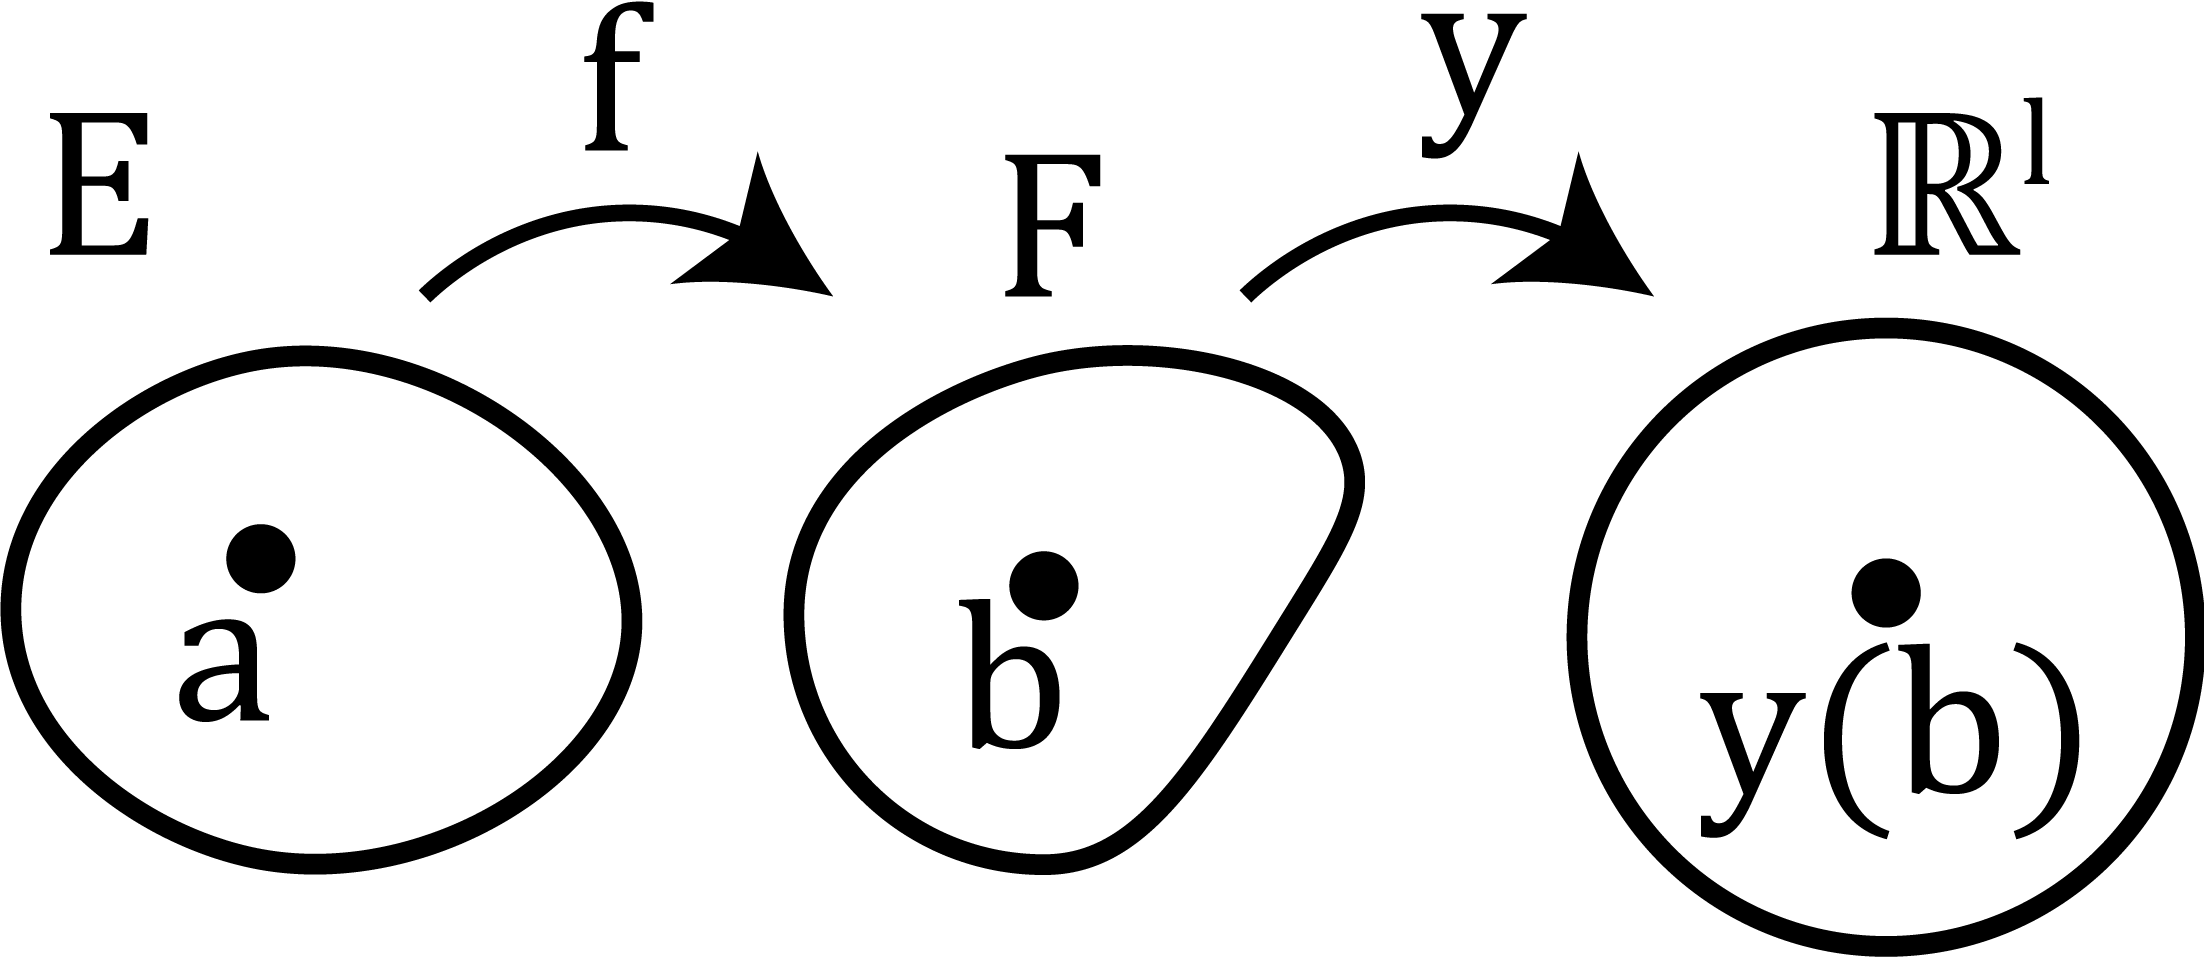
\includegraphics[width=5cm]{pics/2_2}}
		\[\text{ Тогда } \lim_{x \to a} g \circ f = g(b) \]
	\end{Theorem}

	\begin{Theorem}[критерий Коши]
		\[a \text{ --- пред т. } E\]
		\[f(x) \text{ имеет предел в т. } a\]
		\[ \rla \forall \E > 0\q \e \delta > 0 :
			\forall x, y \in\ \doted{U}(a, \delta) \cap E \RA d(f(x), f(y)) < \E\]
	\end{Theorem}

	\begin{Definition} [непрерывные отображения]
		\[a \in E \q\q f: E \to \R^m\]
		Если $a$ --- изол.$\RA f$ --- непр. в $a$\\
		Если $a$ --- пред.$\RA f \text{ --- непр. в т. } a \RLA \displaystyle \lim_{x \to a}f(x) = f(a)$
	\end{Definition}

	\begin{Utv}
		\[f \text{ --- непр. в т.} a \rla f_j \text{ --- непр. в т. } a \ \forall 1 \leq j \leq m\]
		\[f \text{ --- непр. в т. } a,\q g \text{ --- непр. в } f(a) \RLA g \circ f \text{ --- непр. в т } a\]
		\[\text{непр. сохр. при +, умн. на число}\]
		\[f \text{ --- непр. на } E \RLA \text{ непр. } \forall a \in E\]
	\end{Utv}

	\begin{Theorem}[эквивалентность определений непрерывности]
		\[f: E \to \R^m\]
		\[f \text{ --- непр. на } E \rla \forall G \subset \R^m \q G \text{ - откр. } \RA
			f^{-1}(G) \text{ --- откр. в } E\]
	\end{Theorem}

	\begin{proof}
		($\Ra$):
		\[G \text{ --- откр.},\q f^{-1}(G) \text{ --- откр. ?}\]
		\begin{figure}[h!]
			\center{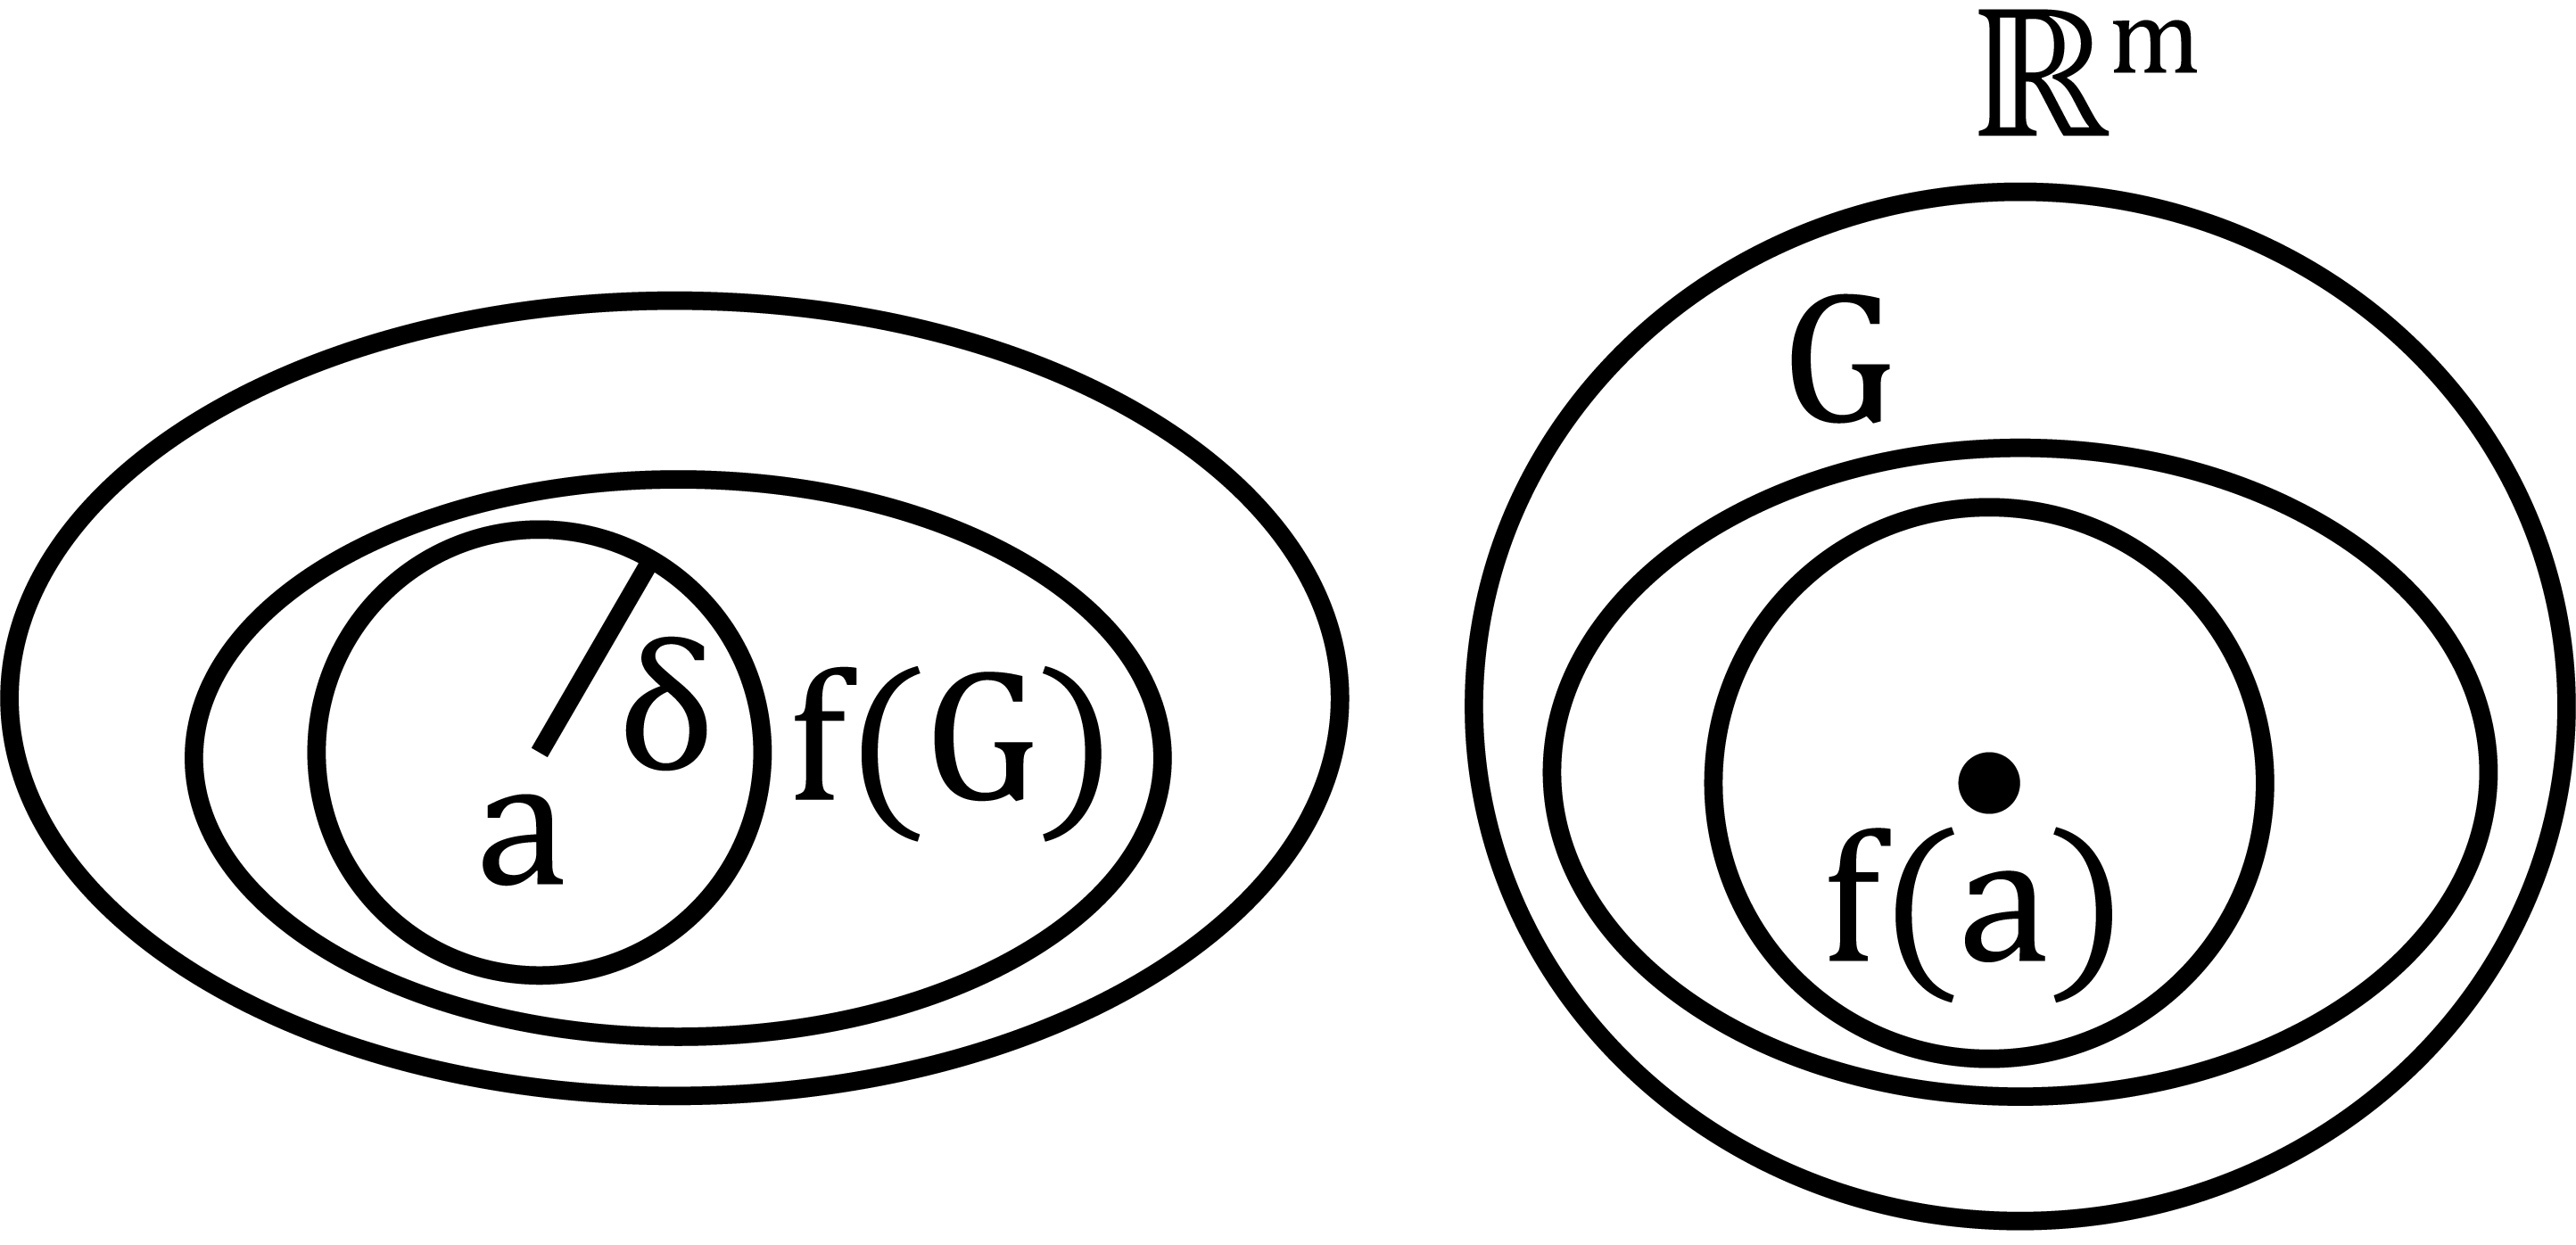
\includegraphics[width = 5.5cm]{pics/2_3}}
		\end{figure}
		\[a \in f^{-1}(G)\]
		\[f(a) \in G \text{ --- откр. } \Ra \e U(f(a), \E) \subset G\]
		\[\text{т.к. } f \text{ непр. в т. } a \q \e \delta : d(a, x) < \delta \Ra d(f(a), f(x)) < \E\]
		\[f(B(a, \delta)) \subset B(f(a), \E) \subset G\]
		\[\Ra B(a, \delta) \subset f^{-1}(G)\]
		($\La$):
		\[a \in E \os{?}{\RA} f \text{ - непр. в т. a}\]
		\begin{figure}[h!]
			\center{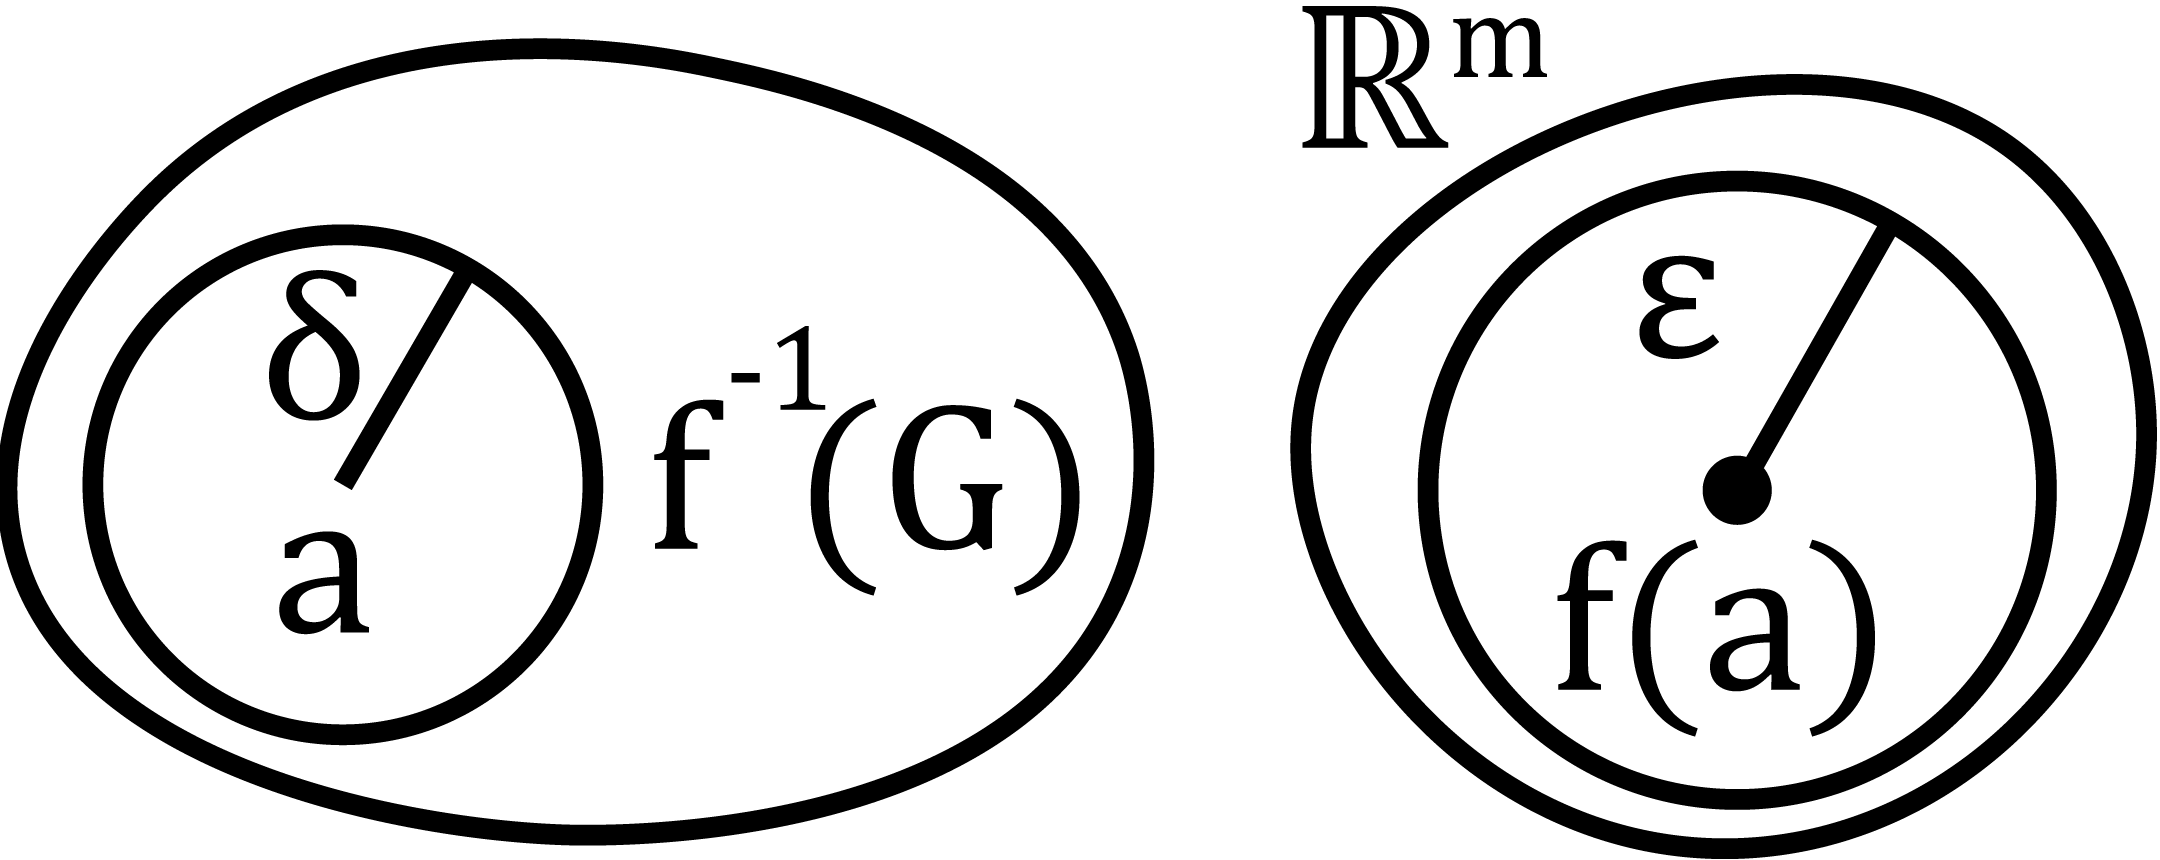
\includegraphics[width = 5cm]{pics/2_4}}
		\end{figure}
		\[\forall \E > 0: B(f(a), \E) \text{ --- откр. в } \R^m \RA f^{-1}(B(f(a), \E) \text{ --- откр.}\]
		\[\Ra \e \delta : B(a, \delta) \subset f^{-1} (B(f(a), \E)) \RA f \text{ --- непр. в т } a\]
	\end{proof}

	\newpage
	\subsection{Локальные и глобальные свойства непрерывных отображений. Доказательство теоремы об образе компакта}

	\begin{theorem}
		\begin{enumerate}
			\item $f$ --- непр. в т. $a \RA f$ --- лок. огр.
			\item $f$ --- непр. в т. $a$, $f(a) > 0 \RA \e$окр. т. a: $f(x) > 0\q \forall x \in U_a$
			\item $f$ --- непр. в т. $a$, $g$ --- непр. в $f(a) \RA g \circ f$ непр. в т. a
		\end{enumerate}
	\end{theorem}
\end{document}
